\section{Data models and formats}

This section gives an overview of the status and plans for the gamma-ray data model and formats. As mentioned before, this effort was only started very recently and none of the formats should be considered stable. The next two sections will describe the effort to define an event data model and format (DL3), and higher-level formats for images, spectra and lightcurves (DL4) (i.e. content split as already illustrated in Figure~\ref{fig:purpose})

In the data specification document we have created a "general" section that gives precise definitions of common quantities, such as precise definitions of time scales as well as coordinates systems. One example is a precise definition of \texttt{AZIMUTH} and \texttt{ALTITUDE}. We define \texttt{AZIMUTH} to be oriented east of north, and \texttt{ALTITUDE} to be relative to the zenith direction (not the horizon plane or a reference earth ellipsoid) and without applying a refraction correction.

There are some general questions we are discussing about where to be specific or flexible in our format specifications. One example is whether our data format specifications should be tied to FITS (and e.g. say the data type of a column is \texttt{1E}, which is the data type code for 32-bit float in FITS), or whether it would be better to only say that the data type is "float", implicitly allowing the storage of this column as 32-bit or 64-bit float, and being able to store the data e.g. in text ECSV files in addition to binary FITS files. Another contentious point is whether physical units should be fixed (e.g. "MeV" or "TeV"), or whether the units should be flexible and only serialization formats that support declaration of units (such as FITS or VOTABLE or ECSV) should be supported and science tools are expected to process the unit information correctly.

\subsection{Data level 3 (DL3) specifications}

The interface between low-level (calibration, reconstruction and gamma-hadron separation pipeline) and high-level (science tool) analysis for gamma-ray data is usually represented by an event list, where at a minimum the \texttt{EVENT\_ID}, observation \texttt{TIME}, as well as the reconstructed \texttt{ENERGY} and sky position (\texttt{RA}, \texttt{DEC}) is given for every event. In addition, instrument response functions (IRFs) as well as auxiliary information such as telescope configuration options, good time intervals (GTIs), livetime and pointing information (collectively called \texttt{TECH} in CTA) are needed by the science tools to compute exposures as well as effective resolutions (PSF and EDISP) and ultimately fluxes and to compare the data with sky models. This DL3 data, illustrated in Figure~\ref{fig:iact-dl3} is similar for all gamma-ray telescopes (and also neutrino telescopes), although in detail it is different e.g. for telescopes that mostly do pointed observations (like IACTs) or that do slewing observations (like Fermi-LAT or HAWC).

\begin{figure}[tb]
\centerline{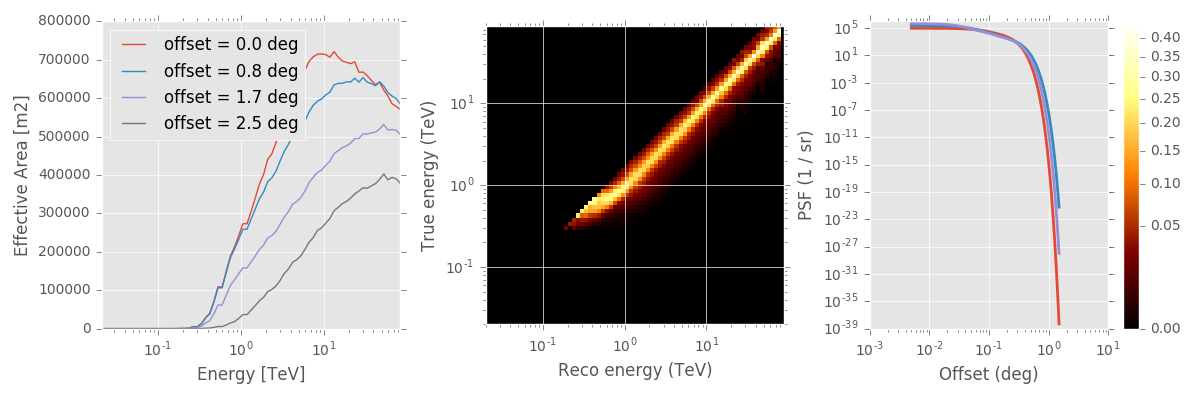
\includegraphics[width=0.9\textwidth]{figures/iact-dl3}}
\caption{
Illustration of major components of IACT ("imaging atmospheric Cherenkov telescope", here a H.E.S.S. 1 Crab nebula observation) DL3 ("data level 3") data. The \texttt{EVENTS} are stored as a table with the most important parameters shown. To derive spectra and morphology measurements of astrophysical sources, IRFs ("instrument response functions") are used: the effective area (\texttt{AEFF}), energy dispersion (\texttt{EDISP}) and point spread function (\texttt{PSF}). Sometimes background (\texttt{BKG}) models are also created and released as part of a DL3 data release, and can be treated like an IRF, and sometimes deriving background models is left to the science tools. Note that this picture is not complete, see the "IACT DL3" section.
}
\label{fig:iact-dl3}
\end{figure}

We have started to develop a data model and format specification for IACT DL3 data. As a starting point, we wrote down the existing formats used by H.E.S.S. and partly also VERITAS and MAGIC, that are mostly supported by the exiting science tool prototypes (Gammapy and ctools). H.E.S.S. is planning to release a small test dataset in the current format consisting of roughly 50 hours of H.E.S.S. 1 observations on a few sources in fall 2016.

A dedicated two-day face-to-face meeting on IACT DL3 data was held in April 2016 in Meudon, France, with 16 participants from all major existing IACTs and CTA (see \ogrameudon). The use cases and status of efforts to export and archive their data in FITS was presented, as well as the ongoing prototyping in science tools. Many important points were discussed, e.g.

\begin{itemize}
\item{}What is an observation? Good time interval? Response time interval?
\item{}How to link \texttt{EVENT} and \texttt{IRF}?
\item{}Pointing and live time information
\item{}IRF axis specification and validity ranges
\item{}FoV coordinates
\item{}How to support multiple EVENT classes and types?
\end{itemize}

A major result of the face-to-face workshop was to agree to focus on IRF formats that use the multi-array convention and FITS BINTABLE to store the IRF data and axis information, where previously a second format was being developed and prototyped for CTA \citep{2015arXiv150807437W}. The prototyping of IACT DL3 is continuing in the different IACT collaborations and in Gammapy/ctools, with communications online via Github, monthly joint tele-conferences, and a planned face-to-face follow-up meeting in fall 2016. So far the focus is on pointed gamma-ray observations, contributions and involvement from people working on slewing telescopes (e.g. Fermi-LAT or HAWC and also IACTs) or non-gamma-ray telescopes with similar data (e.g. neutrino telescopes) are welcome. The largest stakeholder for the IACT DL3 work is CTA.

\subsection{Data level 4 \& 5 specifications}

Another topic in the \texttt{gamma-astro-data-formats} specifications is the development of formats to store high-level data products such as images, spectra or lightcurves (data level 4) or catalog (data level 5).

\begin{itemize}
\item{} For 2-dimensional images, the FITS standard (including world coordinates systems WCS) provides a solution that works for gamma-ray images as well. If something gamma-ray specific were to be added, it would likely be specifications on how to store meta information like the energy band or other analysis or provenance parameters used to make the image.
\item{} For 3-dimensional cubes, where the third dimension is \texttt{ENERGY}, commonly 3-dimensional \texttt{FITS IMAGE} extensions are used. However, due to either the complexity or missing features in the FITS WCS model, the energy axis information is not represented in the FITS header, but a separate \texttt{BINTABLE HDU} instead called \texttt{ENERGY} (if the cube represents quantities at given energies, like exposure or flux), or \texttt{EBOUNDS} ("energy bounds", if the cube represents integral quantities like e.g. counts).
This format has been widely used in gamma-ray astronomy for a long time, a specification at \gadf defining the exact semantics of how the energy axis should be interpolated and integrated would be welcome.
\item{} For all-sky maps and cubes, HEALPIX is commonly used in gamma-ray astronomy (e.g. by Fermi-LAT). While 2-dimensional HEALPIX images are standardized, extensions have been developed to represent cubes, as well as to store sparse data or images that don't cover the whole sky \footnote{\pointlikedata}. These gamma-ray specific extensions are not standardized, and a specification at \gadf would be welcome.
\item{} For 1-dimensional spectra, a format to store flux points and upper limits, as well as full likelihood profiles is available at \gadf (see Figure~\ref{fig:dl4-examples} left panel). It was first developed in Fermipy and applied to Fermi-LAT analyses, and is now being adopted for IACT spectra.
\item{} Lightcurves (see Figure~\ref{fig:dl4-examples} right panel). Description of light curves is another topic open for discussion. Previous work to define a gamma-ray lightcurve format: \cite{2010AnA...524A..48T}
\item{} No format specifications have been proposed for catalogs (data level 5, DL5) yet. So far each catalog (Fermi-LAT, upcoming H.E.S.S. and HAWC) is unique (but all similar) and come science tools have per-catalog code to produce corresponding sky models. Whether it makes sense to try and specify a common catalog format for gamma-ray astronomy remains to be discussed. Probably at least adopting the spectrum and lightcurve formats mentioned before could be useful.
\end{itemize}

\begin{figure}[tb]
\centerline{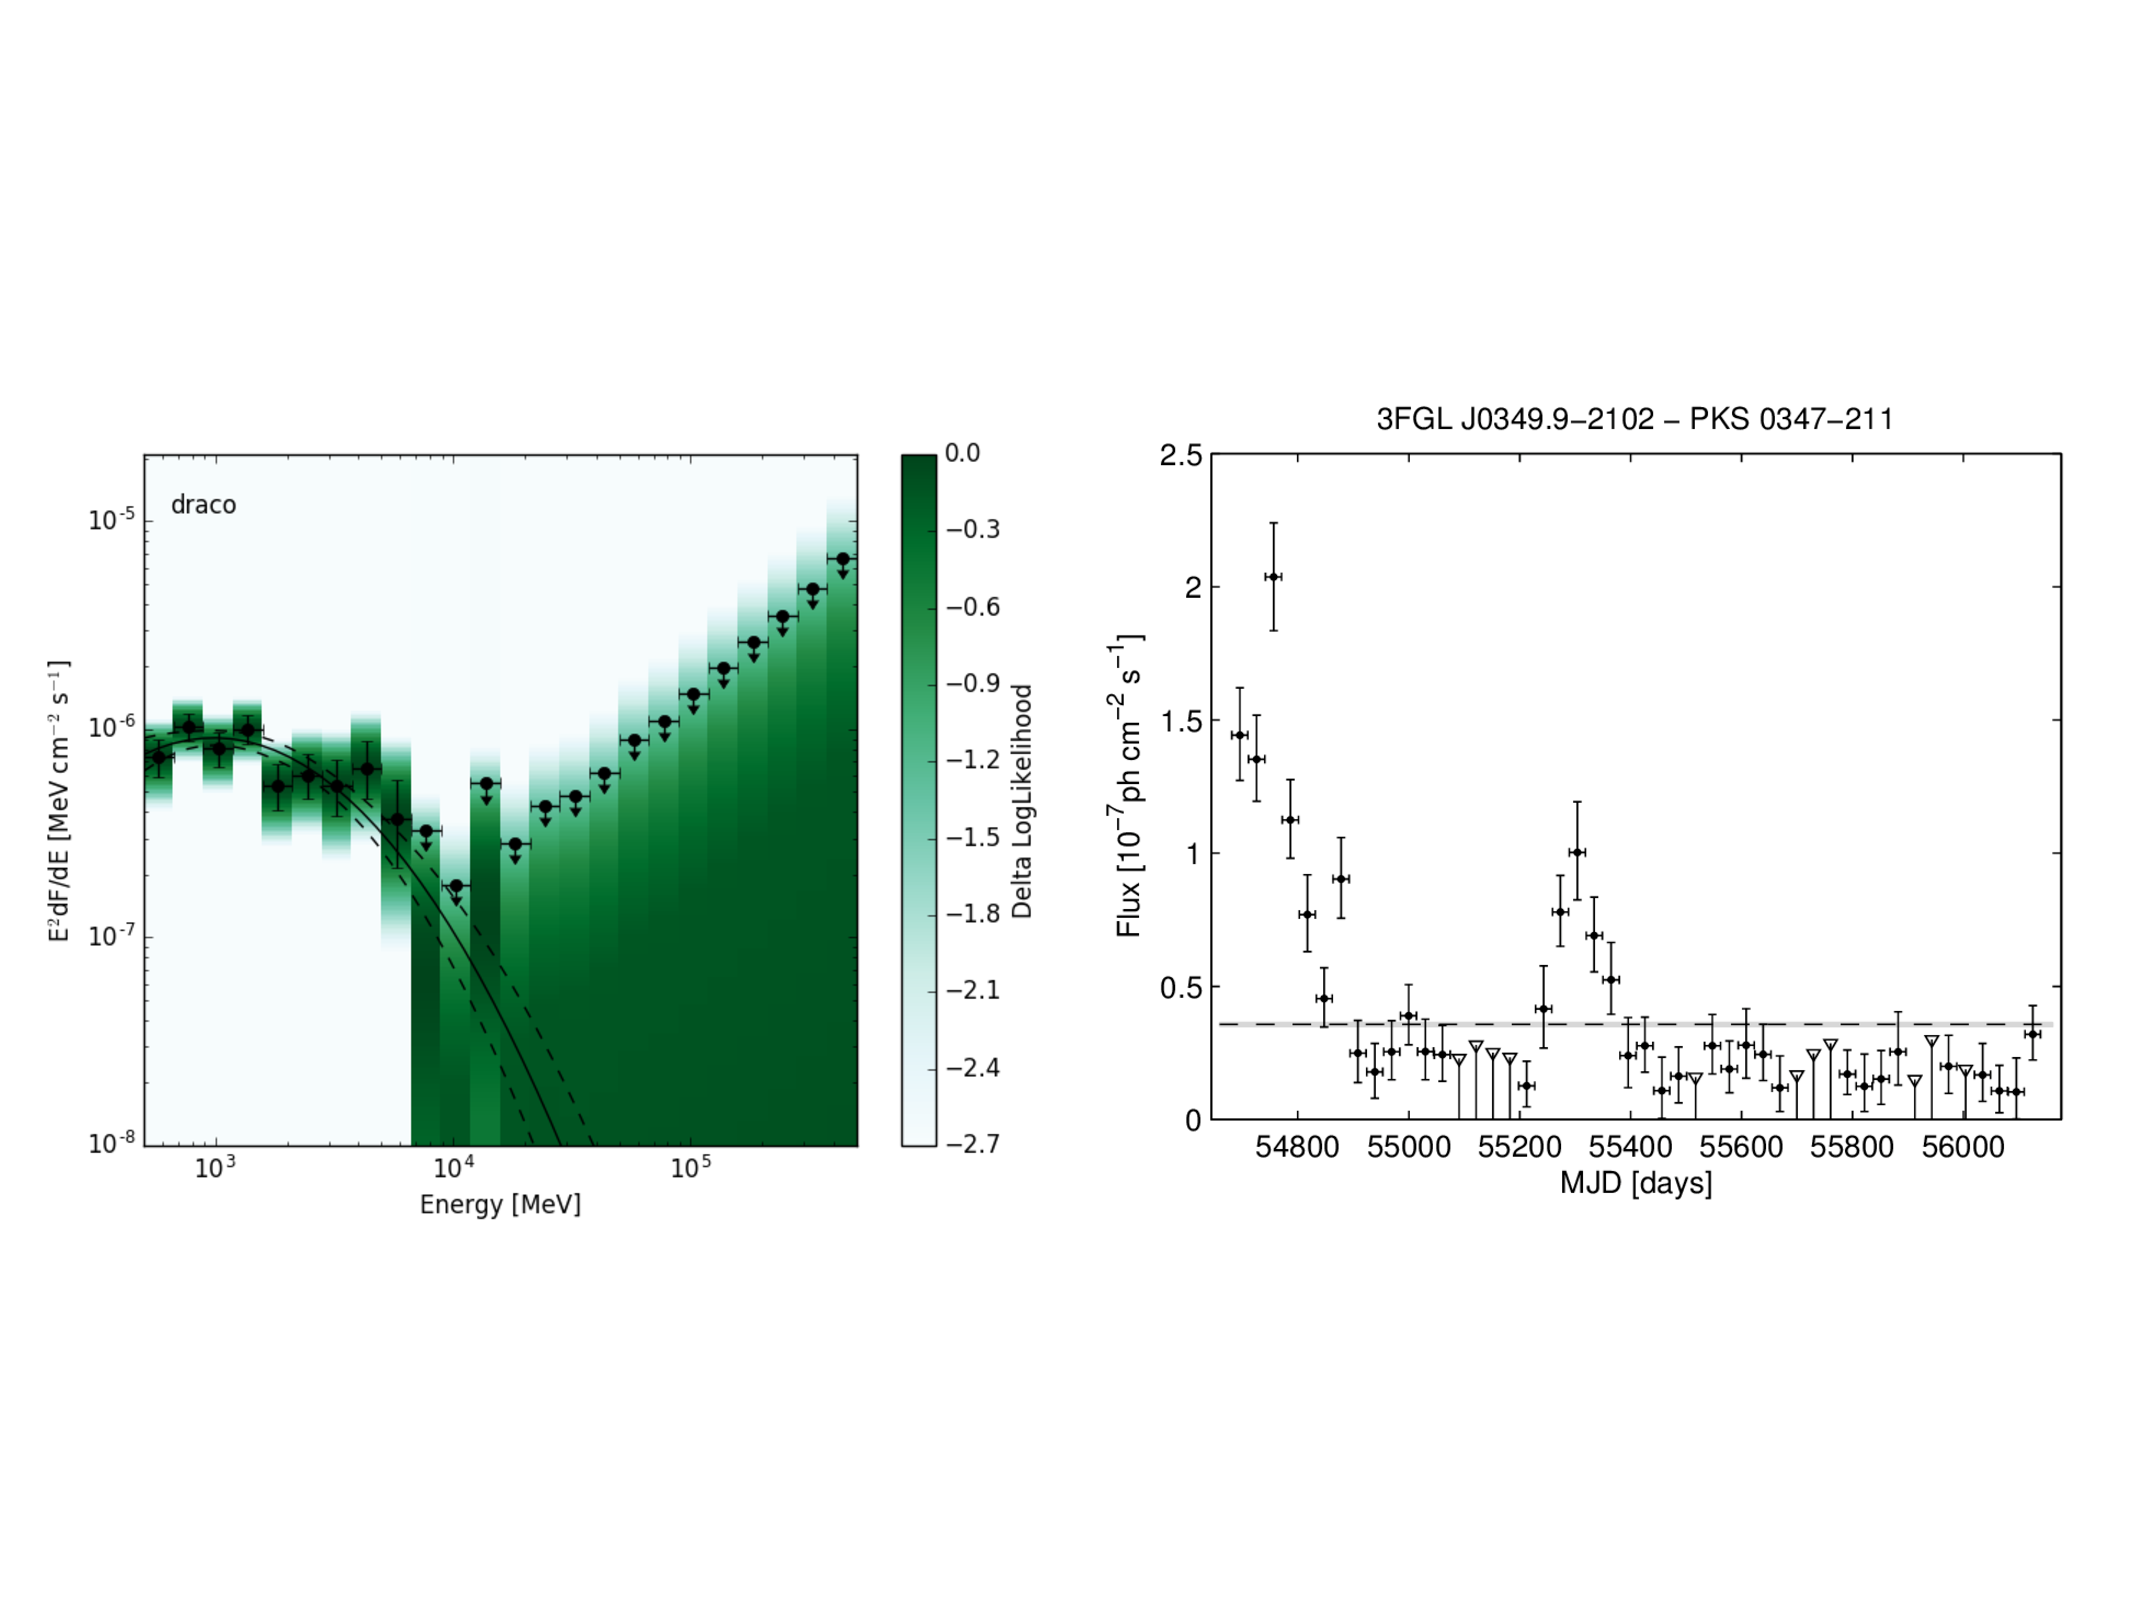
\includegraphics[width=\textwidth]{figures/dl4-examples}}
\caption{
Gamma-ray "data level 4" examples. \emph{Left:} spectral energy distribution (SED) likelihood profiles (green), with flux points and upper limits as well
as a best-model fit overplotted. \emph{Right:} Lightcurve of 3FGL~J0349.9-2102 from the third Fermi-LAT catalog.
}
\label{fig:dl4-examples}
\end{figure}
